\documentclass[1p]{elsarticle_modified}
%\bibliographystyle{elsarticle-num}

%\usepackage[colorlinks]{hyperref}
%\usepackage{abbrmath_seonhwa} %\Abb, \Ascr, \Acal ,\Abf, \Afrak
\usepackage{amsfonts}
\usepackage{amssymb}
\usepackage{amsmath}
\usepackage{amsthm}
\usepackage{scalefnt}
\usepackage{amsbsy}
\usepackage{kotex}
\usepackage{caption}
\usepackage{subfig}
\usepackage{color}
\usepackage{graphicx}
\usepackage{xcolor} %% white, black, red, green, blue, cyan, magenta, yellow
\usepackage{float}
\usepackage{setspace}
\usepackage{hyperref}

\usepackage{tikz}
\usetikzlibrary{arrows}

\usepackage{multirow}
\usepackage{array} % fixed length table
\usepackage{hhline}

%%%%%%%%%%%%%%%%%%%%%
\makeatletter
\renewcommand*\env@matrix[1][\arraystretch]{%
	\edef\arraystretch{#1}%
	\hskip -\arraycolsep
	\let\@ifnextchar\new@ifnextchar
	\array{*\c@MaxMatrixCols c}}
\makeatother %https://tex.stackexchange.com/questions/14071/how-can-i-increase-the-line-spacing-in-a-matrix
%%%%%%%%%%%%%%%

\usepackage[normalem]{ulem}

\newcommand{\msout}[1]{\ifmmode\text{\sout{\ensuremath{#1}}}\else\sout{#1}\fi}
%SOURCE: \msout is \stkout macro in https://tex.stackexchange.com/questions/20609/strikeout-in-math-mode

\newcommand{\cancel}[1]{
	\ifmmode
	{\color{red}\msout{#1}}
	\else
	{\color{red}\sout{#1}}
	\fi
}

\newcommand{\add}[1]{
	{\color{blue}\uwave{#1}}
}

\newcommand{\replace}[2]{
	\ifmmode
	{\color{red}\msout{#1}}{\color{blue}\uwave{#2}}
	\else
	{\color{red}\sout{#1}}{\color{blue}\uwave{#2}}
	\fi
}

\newcommand{\Sol}{\mathcal{S}} %segment
\newcommand{\D}{D} %diagram
\newcommand{\A}{\mathcal{A}} %arc


%%%%%%%%%%%%%%%%%%%%%%%%%%%%%5 test

\def\sl{\operatorname{\textup{SL}}(2,\Cbb)}
\def\psl{\operatorname{\textup{PSL}}(2,\Cbb)}
\def\quan{\mkern 1mu \triangleright \mkern 1mu}

\theoremstyle{definition}
\newtheorem{thm}{Theorem}[section]
\newtheorem{prop}[thm]{Proposition}
\newtheorem{lem}[thm]{Lemma}
\newtheorem{ques}[thm]{Question}
\newtheorem{cor}[thm]{Corollary}
\newtheorem{defn}[thm]{Definition}
\newtheorem{exam}[thm]{Example}
\newtheorem{rmk}[thm]{Remark}
\newtheorem{alg}[thm]{Algorithm}

\newcommand{\I}{\sqrt{-1}}
\begin{document}

%\begin{frontmatter}
%
%\title{Boundary parabolic representations of knots up to 8 crossings}
%
%%% Group authors per affiliation:
%\author{Yunhi Cho} 
%\address{Department of Mathematics, University of Seoul, Seoul, Korea}
%\ead{yhcho@uos.ac.kr}
%
%
%\author{Seonhwa Kim} %\fnref{s_kim}}
%\address{Center for Geometry and Physics, Institute for Basic Science, Pohang, 37673, Korea}
%\ead{ryeona17@ibs.re.kr}
%
%\author{Hyuk Kim}
%\address{Department of Mathematical Sciences, Seoul National University, Seoul 08826, Korea}
%\ead{hyukkim@snu.ac.kr}
%
%\author{Seokbeom Yoon}
%\address{Department of Mathematical Sciences, Seoul National University, Seoul, 08826,  Korea}
%\ead{sbyoon15@snu.ac.kr}
%
%\begin{abstract}
%We find all boundary parabolic representation of knots up to 8 crossings.
%
%\end{abstract}
%\begin{keyword}
%    \MSC[2010] 57M25 
%\end{keyword}
%
%\end{frontmatter}

%\linenumbers
%\tableofcontents
%
\newcommand\colored[1]{\textcolor{white}{\rule[-0.35ex]{0.8em}{1.4ex}}\kern-0.8em\color{red} #1}%
%\newcommand\colored[1]{\textcolor{white}{ #1}\kern-2.17ex	\textcolor{white}{ #1}\kern-1.81ex	\textcolor{white}{ #1}\kern-2.15ex\color{red}#1	}

{\Large $\underline{12a_{0282}~(K12a_{0282})}$}

\setlength{\tabcolsep}{10pt}
\renewcommand{\arraystretch}{1.6}
\vspace{1cm}\begin{tabular}{m{100pt}>{\centering\arraybackslash}m{274pt}}
\multirow{5}{120pt}{
	\centering
	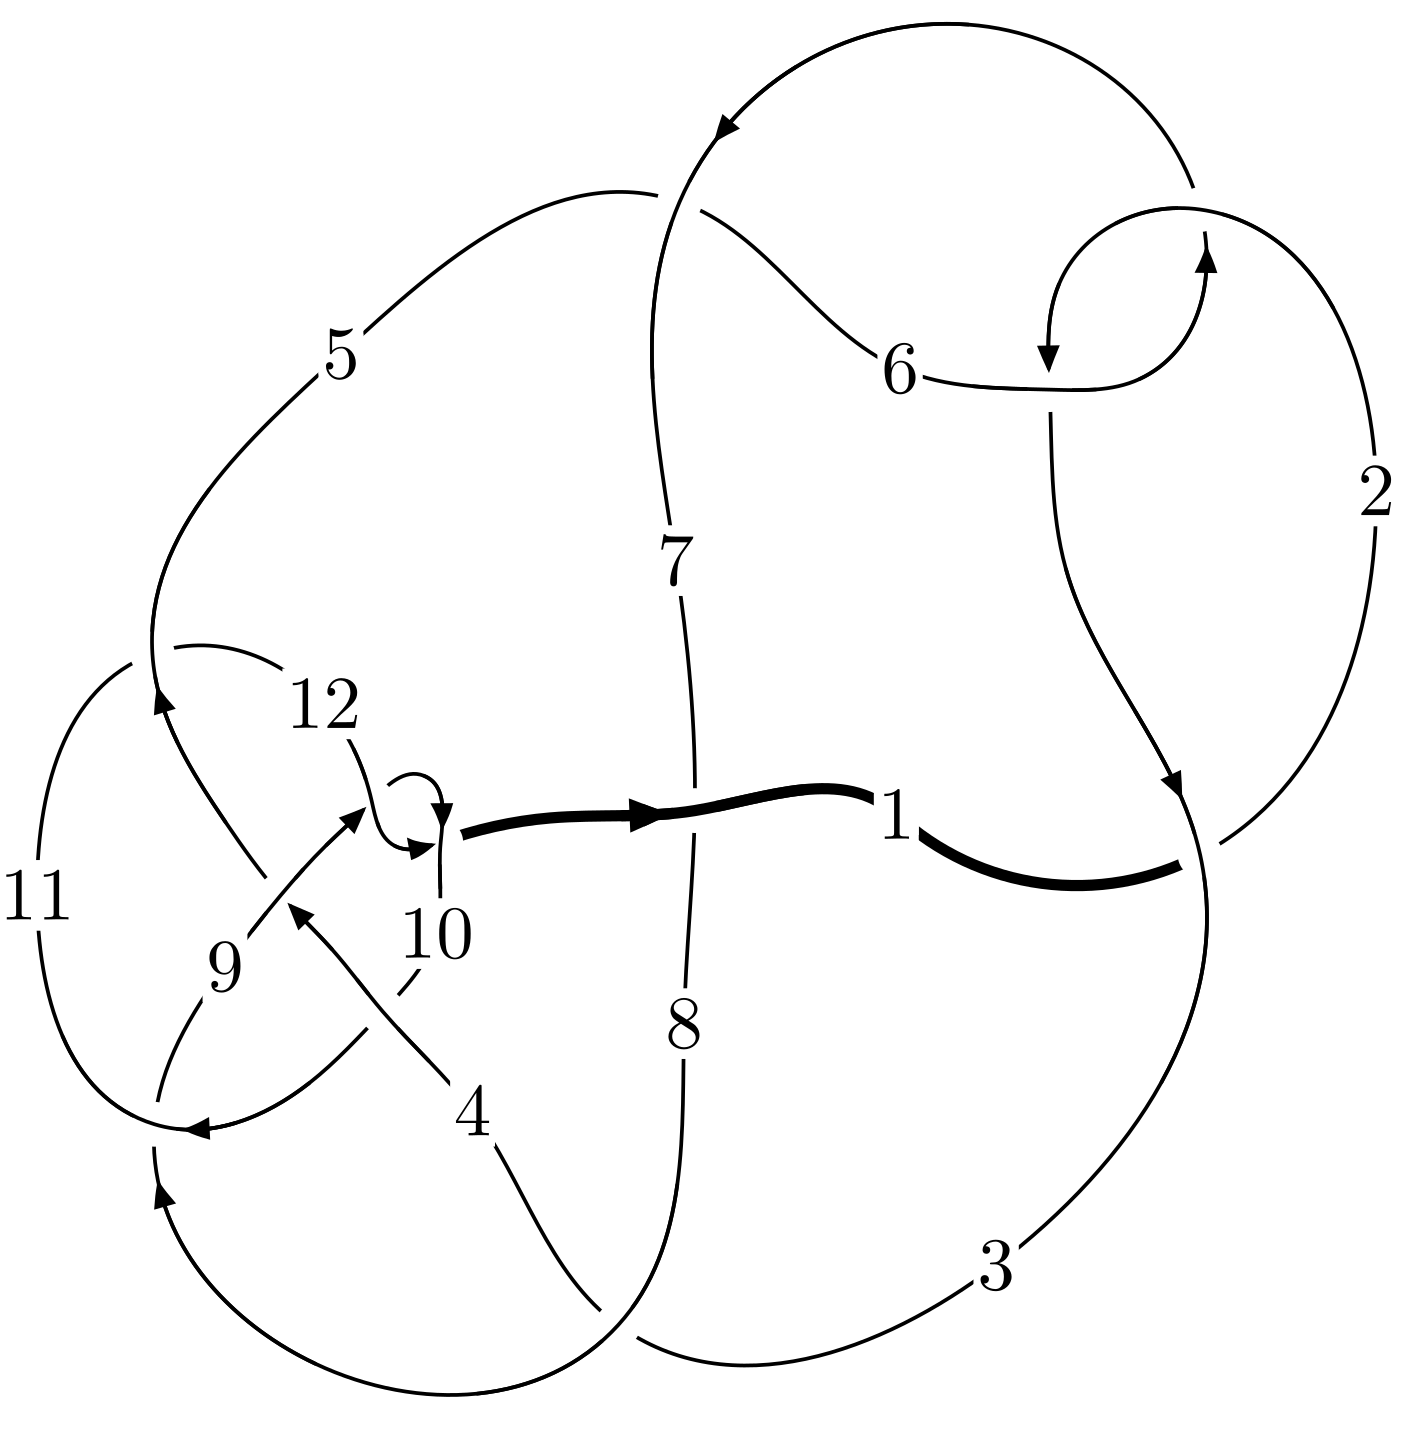
\includegraphics[width=112pt]{../../../GIT/diagram.site/Diagrams/png/1083_12a_0282.png}\\
\ \ \ A knot diagram\footnotemark}&
\allowdisplaybreaks
\textbf{Linearized knot diagam} \\
\cline{2-2}
 &
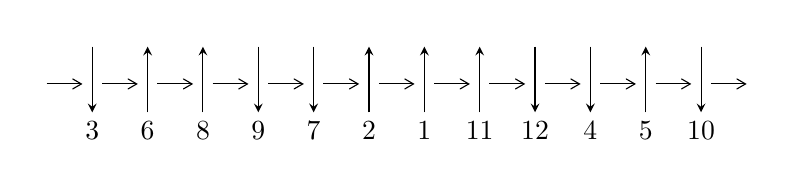
\begin{tikzpicture}[x=20pt, y=17pt]
	% nodes
	\node (C0) at (0, 0) {};
	\node (C1) at (1, 0) {};
	\node (C1U) at (1, +1) {};
	\node (C1D) at (1, -1) {3};

	\node (C2) at (2, 0) {};
	\node (C2U) at (2, +1) {};
	\node (C2D) at (2, -1) {6};

	\node (C3) at (3, 0) {};
	\node (C3U) at (3, +1) {};
	\node (C3D) at (3, -1) {8};

	\node (C4) at (4, 0) {};
	\node (C4U) at (4, +1) {};
	\node (C4D) at (4, -1) {9};

	\node (C5) at (5, 0) {};
	\node (C5U) at (5, +1) {};
	\node (C5D) at (5, -1) {7};

	\node (C6) at (6, 0) {};
	\node (C6U) at (6, +1) {};
	\node (C6D) at (6, -1) {2};

	\node (C7) at (7, 0) {};
	\node (C7U) at (7, +1) {};
	\node (C7D) at (7, -1) {1};

	\node (C8) at (8, 0) {};
	\node (C8U) at (8, +1) {};
	\node (C8D) at (8, -1) {11};

	\node (C9) at (9, 0) {};
	\node (C9U) at (9, +1) {};
	\node (C9D) at (9, -1) {12};

	\node (C10) at (10, 0) {};
	\node (C10U) at (10, +1) {};
	\node (C10D) at (10, -1) {4};

	\node (C11) at (11, 0) {};
	\node (C11U) at (11, +1) {};
	\node (C11D) at (11, -1) {5};

	\node (C12) at (12, 0) {};
	\node (C12U) at (12, +1) {};
	\node (C12D) at (12, -1) {10};
	\node (C13) at (13, 0) {};

	% arrows
	\draw[->,>={angle 60}]
	(C0) edge (C1) (C1) edge (C2) (C2) edge (C3) (C3) edge (C4) (C4) edge (C5) (C5) edge (C6) (C6) edge (C7) (C7) edge (C8) (C8) edge (C9) (C9) edge (C10) (C10) edge (C11) (C11) edge (C12) (C12) edge (C13) ;	\draw[->,>=stealth]
	(C1U) edge (C1D) (C2D) edge (C2U) (C3D) edge (C3U) (C4U) edge (C4D) (C5U) edge (C5D) (C6D) edge (C6U) (C7D) edge (C7U) (C8D) edge (C8U) (C9U) edge (C9D) (C10U) edge (C10D) (C11D) edge (C11U) (C12U) edge (C12D) ;
	\end{tikzpicture} \\
\hhline{~~} \\& 
\textbf{Solving Sequence} \\ \cline{2-2} 
 &
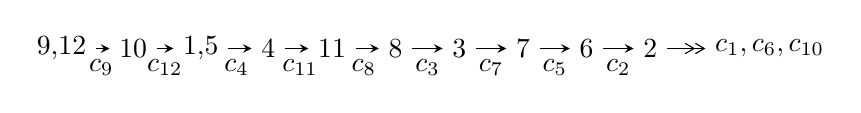
\begin{tikzpicture}[x=23pt, y=7pt]
	% node
	\node (A0) at (-1/8, 0) {9,12};
	\node (A1) at (1, 0) {10};
	\node (A2) at (33/16, 0) {1,5};
	\node (A3) at (25/8, 0) {4};
	\node (A4) at (33/8, 0) {11};
	\node (A5) at (41/8, 0) {8};
	\node (A6) at (49/8, 0) {3};
	\node (A7) at (57/8, 0) {7};
	\node (A8) at (65/8, 0) {6};
	\node (A9) at (73/8, 0) {2};
	\node (C1) at (1/2, -1) {$c_{9}$};
	\node (C2) at (3/2, -1) {$c_{12}$};
	\node (C3) at (21/8, -1) {$c_{4}$};
	\node (C4) at (29/8, -1) {$c_{11}$};
	\node (C5) at (37/8, -1) {$c_{8}$};
	\node (C6) at (45/8, -1) {$c_{3}$};
	\node (C7) at (53/8, -1) {$c_{7}$};
	\node (C8) at (61/8, -1) {$c_{5}$};
	\node (C9) at (69/8, -1) {$c_{2}$};
	\node (A10) at (11, 0) {$c_{1},c_{6},c_{10}$};

	% edge
	\draw[->,>=stealth]	
	(A0) edge (A1) (A1) edge (A2) (A2) edge (A3) (A3) edge (A4) (A4) edge (A5) (A5) edge (A6) (A6) edge (A7) (A7) edge (A8) (A8) edge (A9) ;
	\draw[->>,>={angle 60}]	
	(A9) edge (A10);
\end{tikzpicture} \\ 

\end{tabular} \\

\footnotetext{
The image of knot diagram is generated by the software ``\textbf{Draw programme}" developed by Andrew Bartholomew(\url{http://www.layer8.co.uk/maths/draw/index.htm\#Running-draw}), where we modified some parts for our purpose(\url{https://github.com/CATsTAILs/LinksPainter}).
}\phantom \\ \newline 
\centering \textbf{Ideals for irreducible components\footnotemark of $X_{\text{par}}$} 
 
\begin{align*}
I^u_{1}&=\langle 
-2.07020\times10^{371} u^{117}-5.81468\times10^{371} u^{116}+\cdots+7.49849\times10^{370} b-3.68350\times10^{371},\\
\phantom{I^u_{1}}&\phantom{= \langle  }-3.72284\times10^{371} u^{117}-7.75129\times10^{371} u^{116}+\cdots+7.49849\times10^{370} a-1.71965\times10^{371},\\
\phantom{I^u_{1}}&\phantom{= \langle  }u^{118}+3 u^{117}+\cdots+4 u+1\rangle \\
I^u_{2}&=\langle 
b+a+1,\;a^2+a+1,\;u-1\rangle \\
\\
\end{align*}
\raggedright * 2 irreducible components of $\dim_{\mathbb{C}}=0$, with total 120 representations.\\
\footnotetext{All coefficients of polynomials are rational numbers. But the coefficients are sometimes approximated in decimal forms when there is not enough margin.}
\newpage
\renewcommand{\arraystretch}{1}
\centering \section*{I. $I^u_{1}= \langle -2.07\times10^{371} u^{117}-5.81\times10^{371} u^{116}+\cdots+7.50\times10^{370} b-3.68\times10^{371},\;-3.72\times10^{371} u^{117}-7.75\times10^{371} u^{116}+\cdots+7.50\times10^{370} a-1.72\times10^{371},\;u^{118}+3 u^{117}+\cdots+4 u+1 \rangle$}
\flushleft \textbf{(i) Arc colorings}\\
\begin{tabular}{m{7pt} m{180pt} m{7pt} m{180pt} }
\flushright $a_{9}=$&$\begin{pmatrix}1\\0\end{pmatrix}$ \\
\flushright $a_{12}=$&$\begin{pmatrix}0\\u\end{pmatrix}$ \\
\flushright $a_{10}=$&$\begin{pmatrix}1\\u^2\end{pmatrix}$ \\
\flushright $a_{1}=$&$\begin{pmatrix}- u\\- u^3+u\end{pmatrix}$ \\
\flushright $a_{5}=$&$\begin{pmatrix}4.96478 u^{117}+10.3371 u^{116}+\cdots+2.65024 u+2.29333\\2.76083 u^{117}+7.75447 u^{116}+\cdots+14.8380 u+4.91232\end{pmatrix}$ \\
\flushright $a_{4}=$&$\begin{pmatrix}7.72561 u^{117}+18.0916 u^{116}+\cdots+17.4882 u+7.20565\\2.76083 u^{117}+7.75447 u^{116}+\cdots+14.8380 u+4.91232\end{pmatrix}$ \\
\flushright $a_{11}=$&$\begin{pmatrix}1.65243 u^{117}+3.67747 u^{116}+\cdots+1.68852 u+5.62501\\1.61665 u^{117}+3.65263 u^{116}+\cdots+5.67056 u+2.51293\end{pmatrix}$ \\
\flushright $a_{8}=$&$\begin{pmatrix}0.838669 u^{117}+1.50372 u^{116}+\cdots+3.43379 u+3.79256\\u^3- u\end{pmatrix}$ \\
\flushright $a_{3}=$&$\begin{pmatrix}0.0861580 u^{117}+0.291059 u^{116}+\cdots-11.6079 u+0.298903\\-0.314122 u^{117}+0.483276 u^{116}+\cdots+2.84214 u+1.06374\end{pmatrix}$ \\
\flushright $a_{7}=$&$\begin{pmatrix}0.581121 u^{117}+1.03808 u^{116}+\cdots+2.43549 u+3.53318\\-0.0304212 u^{117}-0.114438 u^{116}+\cdots-0.972145 u-0.0476170\end{pmatrix}$ \\
\flushright $a_{6}=$&$\begin{pmatrix}5.57154 u^{117}+11.8712 u^{116}+\cdots+6.86687 u+2.11380\\0.588302 u^{117}+2.34943 u^{116}+\cdots+6.13446 u+1.92637\end{pmatrix}$ \\
\flushright $a_{2}=$&$\begin{pmatrix}0.0709175 u^{117}+0.593978 u^{116}+\cdots+14.3627 u+4.59643\\-4.77232 u^{117}-9.31946 u^{116}+\cdots-14.1163 u-3.92537\end{pmatrix}$\\&\end{tabular}
\flushleft \textbf{(ii) Obstruction class $= -1$}\\~\\
\flushleft \textbf{(iii) Cusp Shapes $= -26.8874 u^{117}-59.6880 u^{116}+\cdots-86.8976 u-21.2813$}\\~\\
\newpage\renewcommand{\arraystretch}{1}
\flushleft \textbf{(iv) u-Polynomials at the component}\newline \\
\begin{tabular}{m{50pt}|m{274pt}}
Crossings & \hspace{64pt}u-Polynomials at each crossing \\
\hline $$\begin{aligned}c_{1},c_{5}\end{aligned}$$&$\begin{aligned}
&u^{118}+38 u^{117}+\cdots- u+1
\end{aligned}$\\
\hline $$\begin{aligned}c_{2},c_{6}\end{aligned}$$&$\begin{aligned}
&u^{118}-2 u^{117}+\cdots+u+1
\end{aligned}$\\
\hline $$\begin{aligned}c_{3}\end{aligned}$$&$\begin{aligned}
&u^{118}-25 u^{116}+\cdots+7258365 u+2866753
\end{aligned}$\\
\hline $$\begin{aligned}c_{4}\end{aligned}$$&$\begin{aligned}
&u^{118}+4 u^{117}+\cdots+u+1
\end{aligned}$\\
\hline $$\begin{aligned}c_{7}\end{aligned}$$&$\begin{aligned}
&u^{118}+5 u^{117}+\cdots+2784 u+576
\end{aligned}$\\
\hline $$\begin{aligned}c_{8}\end{aligned}$$&$\begin{aligned}
&u^{118}+19 u^{117}+\cdots-4 u+4
\end{aligned}$\\
\hline $$\begin{aligned}c_{9},c_{12}\end{aligned}$$&$\begin{aligned}
&u^{118}-3 u^{117}+\cdots-4 u+1
\end{aligned}$\\
\hline $$\begin{aligned}c_{10}\end{aligned}$$&$\begin{aligned}
&u^{118}+55 u^{116}+\cdots-27 u+1
\end{aligned}$\\
\hline $$\begin{aligned}c_{11}\end{aligned}$$&$\begin{aligned}
&u^{118}+2 u^{117}+\cdots+125 u+71
\end{aligned}$\\
\hline
\end{tabular}\\~\\
\newpage\renewcommand{\arraystretch}{1}
\flushleft \textbf{(v) Riley Polynomials at the component}\newline \\
\begin{tabular}{m{50pt}|m{274pt}}
Crossings & \hspace{64pt}Riley Polynomials at each crossing \\
\hline $$\begin{aligned}c_{1},c_{5}\end{aligned}$$&$\begin{aligned}
&y^{118}+86 y^{117}+\cdots+19 y+1
\end{aligned}$\\
\hline $$\begin{aligned}c_{2},c_{6}\end{aligned}$$&$\begin{aligned}
&y^{118}+38 y^{117}+\cdots- y+1
\end{aligned}$\\
\hline $$\begin{aligned}c_{3}\end{aligned}$$&$\begin{aligned}
&y^{118}-50 y^{117}+\cdots-104190056801433 y+8218272763009
\end{aligned}$\\
\hline $$\begin{aligned}c_{4}\end{aligned}$$&$\begin{aligned}
&y^{118}-18 y^{117}+\cdots- y+1
\end{aligned}$\\
\hline $$\begin{aligned}c_{7}\end{aligned}$$&$\begin{aligned}
&y^{118}-7 y^{117}+\cdots-885888 y+331776
\end{aligned}$\\
\hline $$\begin{aligned}c_{8}\end{aligned}$$&$\begin{aligned}
&y^{118}-15 y^{117}+\cdots-328 y+16
\end{aligned}$\\
\hline $$\begin{aligned}c_{9},c_{12}\end{aligned}$$&$\begin{aligned}
&y^{118}-73 y^{117}+\cdots-56 y+1
\end{aligned}$\\
\hline $$\begin{aligned}c_{10}\end{aligned}$$&$\begin{aligned}
&y^{118}+110 y^{117}+\cdots+111 y+1
\end{aligned}$\\
\hline $$\begin{aligned}c_{11}\end{aligned}$$&$\begin{aligned}
&y^{118}+118 y^{117}+\cdots+457235 y+5041
\end{aligned}$\\
\hline
\end{tabular}\\~\\
\newpage\flushleft \textbf{(vi) Complex Volumes and Cusp Shapes}
$$\begin{array}{c|c|c}  
\text{Solutions to }I^u_{1}& \I (\text{vol} + \sqrt{-1}CS) & \text{Cusp shape}\\
 \hline 
\begin{aligned}
u &= \phantom{-}1.015810 + 0.157426 I \\
a &= \phantom{-}0.38768 + 2.73647 I \\
b &= \phantom{-}0.200813 - 0.493241 I\end{aligned}
 & \phantom{-}2.51659 - 1.87258 I & \phantom{-0.000000 } 0 \\ \hline\begin{aligned}
u &= \phantom{-}1.015810 - 0.157426 I \\
a &= \phantom{-}0.38768 - 2.73647 I \\
b &= \phantom{-}0.200813 + 0.493241 I\end{aligned}
 & \phantom{-}2.51659 + 1.87258 I & \phantom{-0.000000 } 0 \\ \hline\begin{aligned}
u &= \phantom{-}1.029710 + 0.100243 I \\
a &= -0.41457 - 2.87329 I \\
b &= -0.156824 + 0.454000 I\end{aligned}
 & -3.63938 - 2.44452 I & \phantom{-0.000000 } 0 \\ \hline\begin{aligned}
u &= \phantom{-}1.029710 - 0.100243 I \\
a &= -0.41457 + 2.87329 I \\
b &= -0.156824 - 0.454000 I\end{aligned}
 & -3.63938 + 2.44452 I & \phantom{-0.000000 } 0 \\ \hline\begin{aligned}
u &= -1.005490 + 0.266284 I \\
a &= -0.135677 - 0.432659 I \\
b &= \phantom{-}0.79726 + 1.47486 I\end{aligned}
 & -3.26106 + 5.02325 I & \phantom{-0.000000 } 0 \\ \hline\begin{aligned}
u &= -1.005490 - 0.266284 I \\
a &= -0.135677 + 0.432659 I \\
b &= \phantom{-}0.79726 - 1.47486 I\end{aligned}
 & -3.26106 - 5.02325 I & \phantom{-0.000000 } 0 \\ \hline\begin{aligned}
u &= \phantom{-}0.952019 + 0.096599 I \\
a &= \phantom{-}0.59537 + 2.68269 I \\
b &= \phantom{-}0.238554 - 0.415806 I\end{aligned}
 & -0.414651 - 0.426041 I & \phantom{-0.000000 } 0 \\ \hline\begin{aligned}
u &= \phantom{-}0.952019 - 0.096599 I \\
a &= \phantom{-}0.59537 - 2.68269 I \\
b &= \phantom{-}0.238554 + 0.415806 I\end{aligned}
 & -0.414651 + 0.426041 I & \phantom{-0.000000 } 0 \\ \hline\begin{aligned}
u &= \phantom{-}1.032140 + 0.155438 I \\
a &= -0.36475 - 2.75274 I \\
b &= -0.188107 + 0.499728 I\end{aligned}
 & \phantom{-}1.69795 - 7.60447 I & \phantom{-0.000000 } 0 \\ \hline\begin{aligned}
u &= \phantom{-}1.032140 - 0.155438 I \\
a &= -0.36475 + 2.75274 I \\
b &= -0.188107 - 0.499728 I\end{aligned}
 & \phantom{-}1.69795 + 7.60447 I & \phantom{-0.000000 } 0\\
 \hline 
 \end{array}$$\newpage$$\begin{array}{c|c|c}  
\text{Solutions to }I^u_{1}& \I (\text{vol} + \sqrt{-1}CS) & \text{Cusp shape}\\
 \hline 
\begin{aligned}
u &= \phantom{-}0.269115 + 0.917004 I \\
a &= \phantom{-}0.690481 + 0.821341 I \\
b &= -0.687950 - 0.610525 I\end{aligned}
 & \phantom{-}0.02840 - 6.52273 I & \phantom{-0.000000 } 0 \\ \hline\begin{aligned}
u &= \phantom{-}0.269115 - 0.917004 I \\
a &= \phantom{-}0.690481 - 0.821341 I \\
b &= -0.687950 + 0.610525 I\end{aligned}
 & \phantom{-}0.02840 + 6.52273 I & \phantom{-0.000000 } 0 \\ \hline\begin{aligned}
u &= \phantom{-}1.054010 + 0.019013 I \\
a &= -0.14652 - 3.21044 I \\
b &= -0.035898 + 0.412481 I\end{aligned}
 & -1.29395 + 2.39044 I & \phantom{-0.000000 } 0 \\ \hline\begin{aligned}
u &= \phantom{-}1.054010 - 0.019013 I \\
a &= -0.14652 + 3.21044 I \\
b &= -0.035898 - 0.412481 I\end{aligned}
 & -1.29395 - 2.39044 I & \phantom{-0.000000 } 0 \\ \hline\begin{aligned}
u &= -0.901424 + 0.275075 I \\
a &= \phantom{-}0.180834 + 0.360431 I \\
b &= -0.63849 - 1.44278 I\end{aligned}
 & \phantom{-}0.87326 + 2.58349 I & \phantom{-0.000000 } 0 \\ \hline\begin{aligned}
u &= -0.901424 - 0.275075 I \\
a &= \phantom{-}0.180834 - 0.360431 I \\
b &= -0.63849 + 1.44278 I\end{aligned}
 & \phantom{-}0.87326 - 2.58349 I & \phantom{-0.000000 } 0 \\ \hline\begin{aligned}
u &= -1.011000 + 0.354373 I \\
a &= \phantom{-}0.195062 + 0.464782 I \\
b &= -0.79451 - 1.36116 I\end{aligned}
 & \phantom{-}3.39364 + 5.11487 I & \phantom{-0.000000 } 0 \\ \hline\begin{aligned}
u &= -1.011000 - 0.354373 I \\
a &= \phantom{-}0.195062 - 0.464782 I \\
b &= -0.79451 + 1.36116 I\end{aligned}
 & \phantom{-}3.39364 - 5.11487 I & \phantom{-0.000000 } 0 \\ \hline\begin{aligned}
u &= -0.915659 + 0.139482 I \\
a &= -0.074285 - 0.316118 I \\
b &= \phantom{-}0.55915 + 1.72946 I\end{aligned}
 & -1.30357 - 1.42343 I & \phantom{-0.000000 } 0 \\ \hline\begin{aligned}
u &= -0.915659 - 0.139482 I \\
a &= -0.074285 + 0.316118 I \\
b &= \phantom{-}0.55915 - 1.72946 I\end{aligned}
 & -1.30357 + 1.42343 I & \phantom{-0.000000 } 0\\
 \hline 
 \end{array}$$\newpage$$\begin{array}{c|c|c}  
\text{Solutions to }I^u_{1}& \I (\text{vol} + \sqrt{-1}CS) & \text{Cusp shape}\\
 \hline 
\begin{aligned}
u &= -0.081212 + 0.914425 I \\
a &= -0.736305 - 0.669805 I \\
b &= \phantom{-}0.676105 + 0.737768 I\end{aligned}
 & \phantom{-}0.71208 - 1.59697 I & \phantom{-0.000000 } 0 \\ \hline\begin{aligned}
u &= -0.081212 - 0.914425 I \\
a &= -0.736305 + 0.669805 I \\
b &= \phantom{-}0.676105 - 0.737768 I\end{aligned}
 & \phantom{-}0.71208 + 1.59697 I & \phantom{-0.000000 } 0 \\ \hline\begin{aligned}
u &= -0.307163 + 1.040230 I \\
a &= -0.652511 - 0.627322 I \\
b &= \phantom{-}0.735642 + 0.814176 I\end{aligned}
 & \phantom{-}6.57483 + 2.25127 I & \phantom{-0.000000 } 0 \\ \hline\begin{aligned}
u &= -0.307163 - 1.040230 I \\
a &= -0.652511 + 0.627322 I \\
b &= \phantom{-}0.735642 - 0.814176 I\end{aligned}
 & \phantom{-}6.57483 - 2.25127 I & \phantom{-0.000000 } 0 \\ \hline\begin{aligned}
u &= -1.037390 + 0.348408 I \\
a &= -0.183158 - 0.480234 I \\
b &= \phantom{-}0.82330 + 1.36488 I\end{aligned}
 & \phantom{-}2.36107 + 10.94710 I & \phantom{-0.000000 } 0 \\ \hline\begin{aligned}
u &= -1.037390 - 0.348408 I \\
a &= -0.183158 + 0.480234 I \\
b &= \phantom{-}0.82330 - 1.36488 I\end{aligned}
 & \phantom{-}2.36107 - 10.94710 I & \phantom{-0.000000 } 0 \\ \hline\begin{aligned}
u &= -0.281028 + 1.065350 I \\
a &= \phantom{-}0.654000 + 0.637762 I \\
b &= -0.741922 - 0.802911 I\end{aligned}
 & \phantom{-}7.13113 - 3.56996 I & \phantom{-0.000000 } 0 \\ \hline\begin{aligned}
u &= -0.281028 - 1.065350 I \\
a &= \phantom{-}0.654000 - 0.637762 I \\
b &= -0.741922 + 0.802911 I\end{aligned}
 & \phantom{-}7.13113 + 3.56996 I & \phantom{-0.000000 } 0 \\ \hline\begin{aligned}
u &= -0.136691 + 1.096460 I \\
a &= \phantom{-}0.670860 + 0.673006 I \\
b &= -0.743314 - 0.752149 I\end{aligned}
 & \phantom{-}2.97882 - 4.69027 I & \phantom{-0.000000 } 0 \\ \hline\begin{aligned}
u &= -0.136691 - 1.096460 I \\
a &= \phantom{-}0.670860 - 0.673006 I \\
b &= -0.743314 + 0.752149 I\end{aligned}
 & \phantom{-}2.97882 + 4.69027 I & \phantom{-0.000000 } 0\\
 \hline 
 \end{array}$$\newpage$$\begin{array}{c|c|c}  
\text{Solutions to }I^u_{1}& \I (\text{vol} + \sqrt{-1}CS) & \text{Cusp shape}\\
 \hline 
\begin{aligned}
u &= \phantom{-}0.091158 + 0.881469 I \\
a &= -0.752633 - 0.753611 I \\
b &= \phantom{-}0.665671 + 0.671736 I\end{aligned}
 & \phantom{-}0.70380 - 1.66733 I & \phantom{-0.000000 } 0 \\ \hline\begin{aligned}
u &= \phantom{-}0.091158 - 0.881469 I \\
a &= -0.752633 + 0.753611 I \\
b &= \phantom{-}0.665671 - 0.671736 I\end{aligned}
 & \phantom{-}0.70380 + 1.66733 I & \phantom{-0.000000 } 0 \\ \hline\begin{aligned}
u &= \phantom{-}0.861211 + 0.189114 I \\
a &= \phantom{-}0.40154 + 2.54454 I \\
b &= \phantom{-}0.315865 - 0.482426 I\end{aligned}
 & \phantom{-}2.88518 + 0.60480 I & \phantom{-0.000000 } 0 \\ \hline\begin{aligned}
u &= \phantom{-}0.861211 - 0.189114 I \\
a &= \phantom{-}0.40154 - 2.54454 I \\
b &= \phantom{-}0.315865 + 0.482426 I\end{aligned}
 & \phantom{-}2.88518 - 0.60480 I & \phantom{-0.000000 } 0 \\ \hline\begin{aligned}
u &= -0.721420 + 0.496127 I \\
a &= \phantom{-}0.410786 + 0.364333 I \\
b &= -0.601352 - 1.139610 I\end{aligned}
 & \phantom{-}5.78853 + 2.01291 I & \phantom{-0.000000 } 0 \\ \hline\begin{aligned}
u &= -0.721420 - 0.496127 I \\
a &= \phantom{-}0.410786 - 0.364333 I \\
b &= -0.601352 + 1.139610 I\end{aligned}
 & \phantom{-}5.78853 - 2.01291 I & \phantom{-0.000000 } 0 \\ \hline\begin{aligned}
u &= \phantom{-}0.506278 + 0.705306 I \\
a &= \phantom{-}0.592748 + 1.015280 I \\
b &= -0.640262 - 0.510338 I\end{aligned}
 & -3.48678 - 1.44357 I & \phantom{-0.000000 } 0 \\ \hline\begin{aligned}
u &= \phantom{-}0.506278 - 0.705306 I \\
a &= \phantom{-}0.592748 - 1.015280 I \\
b &= -0.640262 + 0.510338 I\end{aligned}
 & -3.48678 + 1.44357 I & \phantom{-0.000000 } 0 \\ \hline\begin{aligned}
u &= -0.667796 + 0.538503 I \\
a &= -0.463899 - 0.369387 I \\
b &= \phantom{-}0.597684 + 1.088240 I\end{aligned}
 & \phantom{-}5.43264 - 3.77865 I & \phantom{-0.000000 } 0 \\ \hline\begin{aligned}
u &= -0.667796 - 0.538503 I \\
a &= -0.463899 + 0.369387 I \\
b &= \phantom{-}0.597684 - 1.088240 I\end{aligned}
 & \phantom{-}5.43264 + 3.77865 I & \phantom{-0.000000 } 0\\
 \hline 
 \end{array}$$\newpage$$\begin{array}{c|c|c}  
\text{Solutions to }I^u_{1}& \I (\text{vol} + \sqrt{-1}CS) & \text{Cusp shape}\\
 \hline 
\begin{aligned}
u &= \phantom{-}0.832730 + 0.200752 I \\
a &= -0.37783 - 2.53219 I \\
b &= -0.332435 + 0.487767 I\end{aligned}
 & \phantom{-}2.16607 + 6.31020 I & \phantom{-0.000000 } 0 \\ \hline\begin{aligned}
u &= \phantom{-}0.832730 - 0.200752 I \\
a &= -0.37783 + 2.53219 I \\
b &= -0.332435 - 0.487767 I\end{aligned}
 & \phantom{-}2.16607 - 6.31020 I & \phantom{-0.000000 } 0 \\ \hline\begin{aligned}
u &= -0.071467 + 1.153040 I \\
a &= -0.663318 - 0.691443 I \\
b &= \phantom{-}0.759544 + 0.728954 I\end{aligned}
 & -0.63375 - 7.11494 I & \phantom{-0.000000 } 0 \\ \hline\begin{aligned}
u &= -0.071467 - 1.153040 I \\
a &= -0.663318 + 0.691443 I \\
b &= \phantom{-}0.759544 - 0.728954 I\end{aligned}
 & -0.63375 + 7.11494 I & \phantom{-0.000000 } 0 \\ \hline\begin{aligned}
u &= -0.739717 + 0.402979 I \\
a &= \phantom{-}1.04982 + 0.97694 I \\
b &= \phantom{-}1.209050 - 0.555868 I\end{aligned}
 & \phantom{-}5.26103 + 7.71157 I & \phantom{-0.000000 } 0 \\ \hline\begin{aligned}
u &= -0.739717 - 0.402979 I \\
a &= \phantom{-}1.04982 - 0.97694 I \\
b &= \phantom{-}1.209050 + 0.555868 I\end{aligned}
 & \phantom{-}5.26103 - 7.71157 I & \phantom{-0.000000 } 0 \\ \hline\begin{aligned}
u &= -0.819019 + 0.155283 I \\
a &= \phantom{-}0.971974 + 0.428416 I \\
b &= \phantom{-}1.54179 - 0.38616 I\end{aligned}
 & -1.21527 + 3.13767 I & \phantom{-0.000000 } 0 \\ \hline\begin{aligned}
u &= -0.819019 - 0.155283 I \\
a &= \phantom{-}0.971974 - 0.428416 I \\
b &= \phantom{-}1.54179 + 0.38616 I\end{aligned}
 & -1.21527 - 3.13767 I & \phantom{-0.000000 } 0 \\ \hline\begin{aligned}
u &= \phantom{-}0.869091 + 0.814784 I \\
a &= \phantom{-}0.361592 + 0.843929 I \\
b &= -0.723955 - 0.412630 I\end{aligned}
 & \phantom{-}1.08187 + 3.26532 I & \phantom{-0.000000 } 0 \\ \hline\begin{aligned}
u &= \phantom{-}0.869091 - 0.814784 I \\
a &= \phantom{-}0.361592 - 0.843929 I \\
b &= -0.723955 + 0.412630 I\end{aligned}
 & \phantom{-}1.08187 - 3.26532 I & \phantom{-0.000000 } 0\\
 \hline 
 \end{array}$$\newpage$$\begin{array}{c|c|c}  
\text{Solutions to }I^u_{1}& \I (\text{vol} + \sqrt{-1}CS) & \text{Cusp shape}\\
 \hline 
\begin{aligned}
u &= -0.134497 + 1.199770 I \\
a &= \phantom{-}0.650884 + 0.682691 I \\
b &= -0.776333 - 0.747087 I\end{aligned}
 & \phantom{-}5.92086 - 6.76139 I & \phantom{-0.000000 } 0 \\ \hline\begin{aligned}
u &= -0.134497 - 1.199770 I \\
a &= \phantom{-}0.650884 - 0.682691 I \\
b &= -0.776333 + 0.747087 I\end{aligned}
 & \phantom{-}5.92086 + 6.76139 I & \phantom{-0.000000 } 0 \\ \hline\begin{aligned}
u &= -0.691973 + 0.382009 I \\
a &= -1.15011 - 0.97644 I \\
b &= -1.188440 + 0.509019 I\end{aligned}
 & \phantom{-}5.89343 + 1.77910 I & \phantom{-0.000000 } 0 \\ \hline\begin{aligned}
u &= -0.691973 - 0.382009 I \\
a &= -1.15011 + 0.97644 I \\
b &= -1.188440 - 0.509019 I\end{aligned}
 & \phantom{-}5.89343 - 1.77910 I & \phantom{-0.000000 } 0 \\ \hline\begin{aligned}
u &= -1.177530 + 0.289452 I \\
a &= \phantom{-}0.406875 + 0.810978 I \\
b &= \phantom{-}1.35862 - 0.97721 I\end{aligned}
 & -2.97221 + 3.73297 I & \phantom{-0.000000 } 0 \\ \hline\begin{aligned}
u &= -1.177530 - 0.289452 I \\
a &= \phantom{-}0.406875 - 0.810978 I \\
b &= \phantom{-}1.35862 + 0.97721 I\end{aligned}
 & -2.97221 - 3.73297 I & \phantom{-0.000000 } 0 \\ \hline\begin{aligned}
u &= -0.118706 + 1.215020 I \\
a &= -0.649535 - 0.686282 I \\
b &= \phantom{-}0.780365 + 0.741648 I\end{aligned}
 & \phantom{-}5.01785 - 12.58190 I & \phantom{-0.000000 } 0 \\ \hline\begin{aligned}
u &= -0.118706 - 1.215020 I \\
a &= -0.649535 + 0.686282 I \\
b &= \phantom{-}0.780365 - 0.741648 I\end{aligned}
 & \phantom{-}5.01785 + 12.58190 I & \phantom{-0.000000 } 0 \\ \hline\begin{aligned}
u &= \phantom{-}0.939468 + 0.789903 I \\
a &= -0.317332 - 0.818773 I \\
b &= \phantom{-}0.728384 + 0.388427 I\end{aligned}
 & \phantom{-}1.72076 - 2.34932 I & \phantom{-0.000000 } 0 \\ \hline\begin{aligned}
u &= \phantom{-}0.939468 - 0.789903 I \\
a &= -0.317332 + 0.818773 I \\
b &= \phantom{-}0.728384 - 0.388427 I\end{aligned}
 & \phantom{-}1.72076 + 2.34932 I & \phantom{-0.000000 } 0\\
 \hline 
 \end{array}$$\newpage$$\begin{array}{c|c|c}  
\text{Solutions to }I^u_{1}& \I (\text{vol} + \sqrt{-1}CS) & \text{Cusp shape}\\
 \hline 
\begin{aligned}
u &= -1.209170 + 0.245411 I \\
a &= -0.352875 - 0.784326 I \\
b &= -1.36271 + 1.02924 I\end{aligned}
 & -4.28002 - 1.46660 I & \phantom{-0.000000 } 0 \\ \hline\begin{aligned}
u &= -1.209170 - 0.245411 I \\
a &= -0.352875 + 0.784326 I \\
b &= -1.36271 - 1.02924 I\end{aligned}
 & -4.28002 + 1.46660 I & \phantom{-0.000000 } 0 \\ \hline\begin{aligned}
u &= \phantom{-}0.757637 + 0.057261 I \\
a &= -0.32575 - 2.30952 I \\
b &= -0.385386 + 0.423671 I\end{aligned}
 & -2.99620 + 1.54111 I & \phantom{-0.000000 } 0 \\ \hline\begin{aligned}
u &= \phantom{-}0.757637 - 0.057261 I \\
a &= -0.32575 + 2.30952 I \\
b &= -0.385386 - 0.423671 I\end{aligned}
 & -2.99620 - 1.54111 I & \phantom{-0.000000 } 0 \\ \hline\begin{aligned}
u &= -1.263400 + 0.317800 I \\
a &= -0.339565 - 0.874731 I \\
b &= -1.29247 + 1.00765 I\end{aligned}
 & -8.36346 + 4.71709 I & \phantom{-0.000000 } 0 \\ \hline\begin{aligned}
u &= -1.263400 - 0.317800 I \\
a &= -0.339565 + 0.874731 I \\
b &= -1.29247 - 1.00765 I\end{aligned}
 & -8.36346 - 4.71709 I & \phantom{-0.000000 } 0 \\ \hline\begin{aligned}
u &= -1.246670 + 0.399816 I \\
a &= \phantom{-}0.381212 + 0.939591 I \\
b &= \phantom{-}1.26177 - 0.96422 I\end{aligned}
 & -3.32751 + 5.96754 I & \phantom{-0.000000 } 0 \\ \hline\begin{aligned}
u &= -1.246670 - 0.399816 I \\
a &= \phantom{-}0.381212 - 0.939591 I \\
b &= \phantom{-}1.26177 + 0.96422 I\end{aligned}
 & -3.32751 - 5.96754 I & \phantom{-0.000000 } 0 \\ \hline\begin{aligned}
u &= \phantom{-}1.308010 + 0.236023 I \\
a &= -0.240272 + 0.391280 I \\
b &= -0.675237 - 0.124696 I\end{aligned}
 & -2.69361 - 0.24186 I & \phantom{-0.000000 } 0 \\ \hline\begin{aligned}
u &= \phantom{-}1.308010 - 0.236023 I \\
a &= -0.240272 - 0.391280 I \\
b &= -0.675237 + 0.124696 I\end{aligned}
 & -2.69361 + 0.24186 I & \phantom{-0.000000 } 0\\
 \hline 
 \end{array}$$\newpage$$\begin{array}{c|c|c}  
\text{Solutions to }I^u_{1}& \I (\text{vol} + \sqrt{-1}CS) & \text{Cusp shape}\\
 \hline 
\begin{aligned}
u &= -1.209850 + 0.589213 I \\
a &= \phantom{-}0.436095 + 1.095500 I \\
b &= \phantom{-}1.17962 - 0.90925 I\end{aligned}
 & \phantom{-}3.70942 + 3.52040 I & \phantom{-0.000000 } 0 \\ \hline\begin{aligned}
u &= -1.209850 - 0.589213 I \\
a &= \phantom{-}0.436095 - 1.095500 I \\
b &= \phantom{-}1.17962 + 0.90925 I\end{aligned}
 & \phantom{-}3.70942 - 3.52040 I & \phantom{-0.000000 } 0 \\ \hline\begin{aligned}
u &= -1.298860 + 0.391525 I \\
a &= -0.335725 - 0.947097 I \\
b &= -1.24676 + 0.98990 I\end{aligned}
 & -4.69083 + 10.88950 I & \phantom{-0.000000 } 0 \\ \hline\begin{aligned}
u &= -1.298860 - 0.391525 I \\
a &= -0.335725 + 0.947097 I \\
b &= -1.24676 - 0.98990 I\end{aligned}
 & -4.69083 - 10.88950 I & \phantom{-0.000000 } 0 \\ \hline\begin{aligned}
u &= \phantom{-}1.190500 + 0.662977 I \\
a &= -0.165168 - 0.676017 I \\
b &= \phantom{-}0.744528 + 0.294187 I\end{aligned}
 & -1.86135 - 2.86516 I & \phantom{-0.000000 } 0 \\ \hline\begin{aligned}
u &= \phantom{-}1.190500 - 0.662977 I \\
a &= -0.165168 + 0.676017 I \\
b &= \phantom{-}0.744528 - 0.294187 I\end{aligned}
 & -1.86135 + 2.86516 I & \phantom{-0.000000 } 0 \\ \hline\begin{aligned}
u &= -1.229850 + 0.596223 I \\
a &= -0.420179 - 1.101220 I \\
b &= -1.17496 + 0.91728 I\end{aligned}
 & \phantom{-}4.12415 + 9.43760 I & \phantom{-0.000000 } 0 \\ \hline\begin{aligned}
u &= -1.229850 - 0.596223 I \\
a &= -0.420179 + 1.101220 I \\
b &= -1.17496 - 0.91728 I\end{aligned}
 & \phantom{-}4.12415 - 9.43760 I & \phantom{-0.000000 } 0 \\ \hline\begin{aligned}
u &= -1.298800 + 0.524744 I \\
a &= \phantom{-}0.362203 + 1.050490 I \\
b &= \phantom{-}1.19470 - 0.95471 I\end{aligned}
 & -3.09034 + 6.91109 I & \phantom{-0.000000 } 0 \\ \hline\begin{aligned}
u &= -1.298800 - 0.524744 I \\
a &= \phantom{-}0.362203 - 1.050490 I \\
b &= \phantom{-}1.19470 + 0.95471 I\end{aligned}
 & -3.09034 - 6.91109 I & \phantom{-0.000000 } 0\\
 \hline 
 \end{array}$$\newpage$$\begin{array}{c|c|c}  
\text{Solutions to }I^u_{1}& \I (\text{vol} + \sqrt{-1}CS) & \text{Cusp shape}\\
 \hline 
\begin{aligned}
u &= -1.30319 + 0.57277 I \\
a &= -0.363552 - 1.086580 I \\
b &= -1.17601 + 0.94880 I\end{aligned}
 & -0.68664 + 10.56830 I & \phantom{-0.000000 } 0 \\ \hline\begin{aligned}
u &= -1.30319 - 0.57277 I \\
a &= -0.363552 + 1.086580 I \\
b &= -1.17601 - 0.94880 I\end{aligned}
 & -0.68664 - 10.56830 I & \phantom{-0.000000 } 0 \\ \hline\begin{aligned}
u &= -0.547763\phantom{ +0.000000I} \\
a &= -1.82067\phantom{ +0.000000I} \\
b &= -1.17013\phantom{ +0.000000I}\end{aligned}
 & \phantom{-}1.89297\phantom{ +0.000000I} & \phantom{-}8.36850\phantom{ +0.000000I} \\ \hline\begin{aligned}
u &= -1.33836 + 0.57259 I \\
a &= \phantom{-}0.338441 + 1.089300 I \\
b &= \phantom{-}1.17117 - 0.96117 I\end{aligned}
 & -4.60882 + 13.13770 I & \phantom{-0.000000 } 0 \\ \hline\begin{aligned}
u &= -1.33836 - 0.57259 I \\
a &= \phantom{-}0.338441 - 1.089300 I \\
b &= \phantom{-}1.17117 + 0.96117 I\end{aligned}
 & -4.60882 - 13.13770 I & \phantom{-0.000000 } 0 \\ \hline\begin{aligned}
u &= -1.33512 + 0.60665 I \\
a &= -0.343160 - 1.112640 I \\
b &= -1.16021 + 0.95569 I\end{aligned}
 & \phantom{-}2.12710 + 13.04790 I & \phantom{-0.000000 } 0 \\ \hline\begin{aligned}
u &= -1.33512 - 0.60665 I \\
a &= -0.343160 + 1.112640 I \\
b &= -1.16021 - 0.95569 I\end{aligned}
 & \phantom{-}2.12710 - 13.04790 I & \phantom{-0.000000 } 0 \\ \hline\begin{aligned}
u &= \phantom{-}1.36618 + 0.55025 I \\
a &= \phantom{-}0.094893 + 0.523038 I \\
b &= -0.763644 - 0.223319 I\end{aligned}
 & -3.28110 + 0.44586 I & \phantom{-0.000000 } 0 \\ \hline\begin{aligned}
u &= \phantom{-}1.36618 - 0.55025 I \\
a &= \phantom{-}0.094893 - 0.523038 I \\
b &= -0.763644 + 0.223319 I\end{aligned}
 & -3.28110 - 0.44586 I & \phantom{-0.000000 } 0 \\ \hline\begin{aligned}
u &= -1.34560 + 0.60651 I \\
a &= \phantom{-}0.335999 + 1.113160 I \\
b &= \phantom{-}1.15904 - 0.95914 I\end{aligned}
 & \phantom{-}1.1409 + 18.9106 I & \phantom{-0.000000 } 0\\
 \hline 
 \end{array}$$\newpage$$\begin{array}{c|c|c}  
\text{Solutions to }I^u_{1}& \I (\text{vol} + \sqrt{-1}CS) & \text{Cusp shape}\\
 \hline 
\begin{aligned}
u &= -1.34560 - 0.60651 I \\
a &= \phantom{-}0.335999 - 1.113160 I \\
b &= \phantom{-}1.15904 + 0.95914 I\end{aligned}
 & \phantom{-}1.1409 - 18.9106 I & \phantom{-0.000000 } 0 \\ \hline\begin{aligned}
u &= \phantom{-}1.30477 + 0.71525 I \\
a &= \phantom{-}0.203861 + 0.593646 I \\
b &= -0.783863 - 0.279163 I\end{aligned}
 & -5.45211 - 4.88189 I & \phantom{-0.000000 } 0 \\ \hline\begin{aligned}
u &= \phantom{-}1.30477 - 0.71525 I \\
a &= \phantom{-}0.203861 - 0.593646 I \\
b &= -0.783863 + 0.279163 I\end{aligned}
 & -5.45211 + 4.88189 I & \phantom{-0.000000 } 0 \\ \hline\begin{aligned}
u &= \phantom{-}1.25456 + 0.80041 I \\
a &= -0.256727 - 0.626353 I \\
b &= \phantom{-}0.791903 + 0.309346 I\end{aligned}
 & \phantom{-}0.76439 - 4.56010 I & \phantom{-0.000000 } 0 \\ \hline\begin{aligned}
u &= \phantom{-}1.25456 - 0.80041 I \\
a &= -0.256727 + 0.626353 I \\
b &= \phantom{-}0.791903 - 0.309346 I\end{aligned}
 & \phantom{-}0.76439 + 4.56010 I & \phantom{-0.000000 } 0 \\ \hline\begin{aligned}
u &= \phantom{-}1.44617 + 0.44415 I \\
a &= -0.046547 - 0.422137 I \\
b &= \phantom{-}0.766830 + 0.175809 I\end{aligned}
 & -3.50011 - 4.05313 I & \phantom{-0.000000 } 0 \\ \hline\begin{aligned}
u &= \phantom{-}1.44617 - 0.44415 I \\
a &= -0.046547 + 0.422137 I \\
b &= \phantom{-}0.766830 - 0.175809 I\end{aligned}
 & -3.50011 + 4.05313 I & \phantom{-0.000000 } 0 \\ \hline\begin{aligned}
u &= \phantom{-}1.28308 + 0.80664 I \\
a &= \phantom{-}0.259937 + 0.609495 I \\
b &= -0.799316 - 0.304270 I\end{aligned}
 & -0.12251 - 10.28450 I & \phantom{-0.000000 } 0 \\ \hline\begin{aligned}
u &= \phantom{-}1.28308 - 0.80664 I \\
a &= \phantom{-}0.259937 - 0.609495 I \\
b &= -0.799316 + 0.304270 I\end{aligned}
 & -0.12251 + 10.28450 I & \phantom{-0.000000 } 0 \\ \hline\begin{aligned}
u &= -0.283331 + 0.365958 I \\
a &= -1.89931 - 1.77238 I \\
b &= -0.856366 + 0.377788 I\end{aligned}
 & \phantom{-}5.29542 - 1.89909 I & \phantom{-}5.77474 - 1.14352 I\\
 \hline 
 \end{array}$$\newpage$$\begin{array}{c|c|c}  
\text{Solutions to }I^u_{1}& \I (\text{vol} + \sqrt{-1}CS) & \text{Cusp shape}\\
 \hline 
\begin{aligned}
u &= -0.283331 - 0.365958 I \\
a &= -1.89931 + 1.77238 I \\
b &= -0.856366 - 0.377788 I\end{aligned}
 & \phantom{-}5.29542 + 1.89909 I & \phantom{-}5.77474 + 1.14352 I \\ \hline\begin{aligned}
u &= -0.242525 + 0.384233 I \\
a &= \phantom{-}1.86328 + 1.93677 I \\
b &= \phantom{-}0.824641 - 0.392540 I\end{aligned}
 & \phantom{-}4.46807 - 7.74602 I & \phantom{-}4.03411 + 3.90401 I \\ \hline\begin{aligned}
u &= -0.242525 - 0.384233 I \\
a &= \phantom{-}1.86328 - 1.93677 I \\
b &= \phantom{-}0.824641 + 0.392540 I\end{aligned}
 & \phantom{-}4.46807 + 7.74602 I & \phantom{-}4.03411 - 3.90401 I \\ \hline\begin{aligned}
u &= \phantom{-}1.52175 + 0.29164 I \\
a &= \phantom{-}0.002981 - 0.278462 I \\
b &= \phantom{-}0.768917 + 0.113049 I\end{aligned}
 & -6.23740 + 1.19915 I & \phantom{-0.000000 } 0 \\ \hline\begin{aligned}
u &= \phantom{-}1.52175 - 0.29164 I \\
a &= \phantom{-}0.002981 + 0.278462 I \\
b &= \phantom{-}0.768917 - 0.113049 I\end{aligned}
 & -6.23740 - 1.19915 I & \phantom{-0.000000 } 0 \\ \hline\begin{aligned}
u &= \phantom{-}1.58291 + 0.16873 I \\
a &= -0.005354 + 0.153580 I \\
b &= -0.779064 - 0.062993 I\end{aligned}
 & -0.396545 + 0.829721 I & \phantom{-0.000000 } 0 \\ \hline\begin{aligned}
u &= \phantom{-}1.58291 - 0.16873 I \\
a &= -0.005354 - 0.153580 I \\
b &= -0.779064 + 0.062993 I\end{aligned}
 & -0.396545 - 0.829721 I & \phantom{-0.000000 } 0 \\ \hline\begin{aligned}
u &= -0.400507\phantom{ +0.000000I} \\
a &= -2.48892\phantom{ +0.000000I} \\
b &= -0.983507\phantom{ +0.000000I}\end{aligned}
 & \phantom{-}1.89645\phantom{ +0.000000I} & \phantom{-}7.34120\phantom{ +0.000000I} \\ \hline\begin{aligned}
u &= \phantom{-}1.60558 + 0.20241 I \\
a &= -0.023615 - 0.173894 I \\
b &= \phantom{-}0.789565 + 0.073334 I\end{aligned}
 & -1.22456 + 6.46109 I & \phantom{-0.000000 } 0 \\ \hline\begin{aligned}
u &= \phantom{-}1.60558 - 0.20241 I \\
a &= -0.023615 + 0.173894 I \\
b &= \phantom{-}0.789565 - 0.073334 I\end{aligned}
 & -1.22456 - 6.46109 I & \phantom{-0.000000 } 0\\
 \hline 
 \end{array}$$\newpage$$\begin{array}{c|c|c}  
\text{Solutions to }I^u_{1}& \I (\text{vol} + \sqrt{-1}CS) & \text{Cusp shape}\\
 \hline 
\begin{aligned}
u &= -0.049857 + 0.375700 I \\
a &= -1.42763 - 0.44078 I \\
b &= \phantom{-}0.412152 + 0.687938 I\end{aligned}
 & \phantom{-}0.236053 - 1.263220 I & \phantom{-}2.77957 + 4.87921 I \\ \hline\begin{aligned}
u &= -0.049857 - 0.375700 I \\
a &= -1.42763 + 0.44078 I \\
b &= \phantom{-}0.412152 - 0.687938 I\end{aligned}
 & \phantom{-}0.236053 + 1.263220 I & \phantom{-}2.77957 - 4.87921 I \\ \hline\begin{aligned}
u &= \phantom{-}0.344749 + 0.071658 I \\
a &= \phantom{-}0.37116 - 3.05567 I \\
b &= -0.460452 + 0.450709 I\end{aligned}
 & \phantom{-}0.10228 - 2.99479 I & -1.46599 + 2.14432 I \\ \hline\begin{aligned}
u &= \phantom{-}0.344749 - 0.071658 I \\
a &= \phantom{-}0.37116 + 3.05567 I \\
b &= -0.460452 - 0.450709 I\end{aligned}
 & \phantom{-}0.10228 + 2.99479 I & -1.46599 - 2.14432 I \\ \hline\begin{aligned}
u &= -0.150353 + 0.230107 I \\
a &= \phantom{-}2.76365 + 2.39774 I \\
b &= \phantom{-}0.727149 - 0.276598 I\end{aligned}
 & -1.28119 - 2.58393 I & -1.57512 + 2.81813 I \\ \hline\begin{aligned}
u &= -0.150353 - 0.230107 I \\
a &= \phantom{-}2.76365 - 2.39774 I \\
b &= \phantom{-}0.727149 + 0.276598 I\end{aligned}
 & -1.28119 + 2.58393 I & -1.57512 - 2.81813 I \\ \hline\begin{aligned}
u &= \phantom{-}0.179612 + 0.093018 I \\
a &= -0.35158 + 4.28461 I \\
b &= \phantom{-}0.463286 - 0.401306 I\end{aligned}
 & \phantom{-}0.40695 + 1.93439 I & -0.33283 - 3.61891 I \\ \hline\begin{aligned}
u &= \phantom{-}0.179612 - 0.093018 I \\
a &= -0.35158 - 4.28461 I \\
b &= \phantom{-}0.463286 + 0.401306 I\end{aligned}
 & \phantom{-}0.40695 - 1.93439 I & -0.33283 + 3.61891 I\\
 \hline 
 \end{array}$$\newpage\newpage\renewcommand{\arraystretch}{1}
\centering \section*{II. $I^u_{2}= \langle b+a+1,\;a^2+a+1,\;u-1 \rangle$}
\flushleft \textbf{(i) Arc colorings}\\
\begin{tabular}{m{7pt} m{180pt} m{7pt} m{180pt} }
\flushright $a_{9}=$&$\begin{pmatrix}1\\0\end{pmatrix}$ \\
\flushright $a_{12}=$&$\begin{pmatrix}0\\1\end{pmatrix}$ \\
\flushright $a_{10}=$&$\begin{pmatrix}1\\1\end{pmatrix}$ \\
\flushright $a_{1}=$&$\begin{pmatrix}-1\\0\end{pmatrix}$ \\
\flushright $a_{5}=$&$\begin{pmatrix}a\\- a-1\end{pmatrix}$ \\
\flushright $a_{4}=$&$\begin{pmatrix}-1\\- a-1\end{pmatrix}$ \\
\flushright $a_{11}=$&$\begin{pmatrix}a+1\\0\end{pmatrix}$ \\
\flushright $a_{8}=$&$\begin{pmatrix}1\\0\end{pmatrix}$ \\
\flushright $a_{3}=$&$\begin{pmatrix}a\\- a-1\end{pmatrix}$ \\
\flushright $a_{7}=$&$\begin{pmatrix}1\\0\end{pmatrix}$ \\
\flushright $a_{6}=$&$\begin{pmatrix}2 a+1\\- a-1\end{pmatrix}$ \\
\flushright $a_{2}=$&$\begin{pmatrix}-2\\- a\end{pmatrix}$\\&\end{tabular}
\flushleft \textbf{(ii) Obstruction class $= 1$}\\~\\
\flushleft \textbf{(iii) Cusp Shapes $= 4 a-1$}\\~\\
\newpage\renewcommand{\arraystretch}{1}
\flushleft \textbf{(iv) u-Polynomials at the component}\newline \\
\begin{tabular}{m{50pt}|m{274pt}}
Crossings & \hspace{64pt}u-Polynomials at each crossing \\
\hline $$\begin{aligned}c_{1},c_{3},c_{4}\\c_{5},c_{6},c_{10}\\c_{11}\end{aligned}$$&$\begin{aligned}
&u^2- u+1
\end{aligned}$\\
\hline $$\begin{aligned}c_{2}\end{aligned}$$&$\begin{aligned}
&u^2+u+1
\end{aligned}$\\
\hline $$\begin{aligned}c_{7},c_{8}\end{aligned}$$&$\begin{aligned}
&u^2
\end{aligned}$\\
\hline $$\begin{aligned}c_{9}\end{aligned}$$&$\begin{aligned}
&(u-1)^2
\end{aligned}$\\
\hline $$\begin{aligned}c_{12}\end{aligned}$$&$\begin{aligned}
&(u+1)^2
\end{aligned}$\\
\hline
\end{tabular}\\~\\
\newpage\renewcommand{\arraystretch}{1}
\flushleft \textbf{(v) Riley Polynomials at the component}\newline \\
\begin{tabular}{m{50pt}|m{274pt}}
Crossings & \hspace{64pt}Riley Polynomials at each crossing \\
\hline $$\begin{aligned}c_{1},c_{2},c_{3}\\c_{4},c_{5},c_{6}\\c_{10},c_{11}\end{aligned}$$&$\begin{aligned}
&y^2+y+1
\end{aligned}$\\
\hline $$\begin{aligned}c_{7},c_{8}\end{aligned}$$&$\begin{aligned}
&y^2
\end{aligned}$\\
\hline $$\begin{aligned}c_{9},c_{12}\end{aligned}$$&$\begin{aligned}
&(y-1)^2
\end{aligned}$\\
\hline
\end{tabular}\\~\\
\newpage\flushleft \textbf{(vi) Complex Volumes and Cusp Shapes}
$$\begin{array}{c|c|c}  
\text{Solutions to }I^u_{2}& \I (\text{vol} + \sqrt{-1}CS) & \text{Cusp shape}\\
 \hline 
\begin{aligned}
u &= \phantom{-}1.00000\phantom{ +0.000000I} \\
a &= -0.500000 + 0.866025 I \\
b &= -0.500000 - 0.866025 I\end{aligned}
 & -1.64493 - 2.02988 I & -3.00000 + 3.46410 I \\ \hline\begin{aligned}
u &= \phantom{-}1.00000\phantom{ +0.000000I} \\
a &= -0.500000 - 0.866025 I \\
b &= -0.500000 + 0.866025 I\end{aligned}
 & -1.64493 + 2.02988 I & -3.00000 - 3.46410 I\\
 \hline 
 \end{array}$$\newpage
\newpage\renewcommand{\arraystretch}{1}
\centering \section*{ III. u-Polynomials}
\begin{tabular}{m{50pt}|m{274pt}}
Crossings & \hspace{64pt}u-Polynomials at each crossing \\
\hline $$\begin{aligned}c_{1},c_{5}\end{aligned}$$&$\begin{aligned}
&(u^2- u+1)(u^{118}+38 u^{117}+\cdots- u+1)
\end{aligned}$\\
\hline $$\begin{aligned}c_{2}\end{aligned}$$&$\begin{aligned}
&(u^2+u+1)(u^{118}-2 u^{117}+\cdots+u+1)
\end{aligned}$\\
\hline $$\begin{aligned}c_{3}\end{aligned}$$&$\begin{aligned}
&(u^2- u+1)(u^{118}-25 u^{116}+\cdots+7258365 u+2866753)
\end{aligned}$\\
\hline $$\begin{aligned}c_{4}\end{aligned}$$&$\begin{aligned}
&(u^2- u+1)(u^{118}+4 u^{117}+\cdots+u+1)
\end{aligned}$\\
\hline $$\begin{aligned}c_{6}\end{aligned}$$&$\begin{aligned}
&(u^2- u+1)(u^{118}-2 u^{117}+\cdots+u+1)
\end{aligned}$\\
\hline $$\begin{aligned}c_{7}\end{aligned}$$&$\begin{aligned}
&u^2(u^{118}+5 u^{117}+\cdots+2784 u+576)
\end{aligned}$\\
\hline $$\begin{aligned}c_{8}\end{aligned}$$&$\begin{aligned}
&u^2(u^{118}+19 u^{117}+\cdots-4 u+4)
\end{aligned}$\\
\hline $$\begin{aligned}c_{9}\end{aligned}$$&$\begin{aligned}
&((u-1)^2)(u^{118}-3 u^{117}+\cdots-4 u+1)
\end{aligned}$\\
\hline $$\begin{aligned}c_{10}\end{aligned}$$&$\begin{aligned}
&(u^2- u+1)(u^{118}+55 u^{116}+\cdots-27 u+1)
\end{aligned}$\\
\hline $$\begin{aligned}c_{11}\end{aligned}$$&$\begin{aligned}
&(u^2- u+1)(u^{118}+2 u^{117}+\cdots+125 u+71)
\end{aligned}$\\
\hline $$\begin{aligned}c_{12}\end{aligned}$$&$\begin{aligned}
&((u+1)^2)(u^{118}-3 u^{117}+\cdots-4 u+1)
\end{aligned}$\\
\hline
\end{tabular}\newpage\renewcommand{\arraystretch}{1}
\centering \section*{ IV. Riley Polynomials}
\begin{tabular}{m{50pt}|m{274pt}}
Crossings & \hspace{64pt}Riley Polynomials at each crossing \\
\hline $$\begin{aligned}c_{1},c_{5}\end{aligned}$$&$\begin{aligned}
&(y^2+y+1)(y^{118}+86 y^{117}+\cdots+19 y+1)
\end{aligned}$\\
\hline $$\begin{aligned}c_{2},c_{6}\end{aligned}$$&$\begin{aligned}
&(y^2+y+1)(y^{118}+38 y^{117}+\cdots- y+1)
\end{aligned}$\\
\hline $$\begin{aligned}c_{3}\end{aligned}$$&$\begin{aligned}
&(y^2+y+1)\\
&\cdot(y^{118}-50 y^{117}+\cdots-104190056801433 y+8218272763009)
\end{aligned}$\\
\hline $$\begin{aligned}c_{4}\end{aligned}$$&$\begin{aligned}
&(y^2+y+1)(y^{118}-18 y^{117}+\cdots- y+1)
\end{aligned}$\\
\hline $$\begin{aligned}c_{7}\end{aligned}$$&$\begin{aligned}
&y^2(y^{118}-7 y^{117}+\cdots-885888 y+331776)
\end{aligned}$\\
\hline $$\begin{aligned}c_{8}\end{aligned}$$&$\begin{aligned}
&y^2(y^{118}-15 y^{117}+\cdots-328 y+16)
\end{aligned}$\\
\hline $$\begin{aligned}c_{9},c_{12}\end{aligned}$$&$\begin{aligned}
&((y-1)^2)(y^{118}-73 y^{117}+\cdots-56 y+1)
\end{aligned}$\\
\hline $$\begin{aligned}c_{10}\end{aligned}$$&$\begin{aligned}
&(y^2+y+1)(y^{118}+110 y^{117}+\cdots+111 y+1)
\end{aligned}$\\
\hline $$\begin{aligned}c_{11}\end{aligned}$$&$\begin{aligned}
&(y^2+y+1)(y^{118}+118 y^{117}+\cdots+457235 y+5041)
\end{aligned}$\\
\hline
\end{tabular}
\vskip 2pc
\end{document}